\appendix

\section{Experiment 1 Methods}
\subsection{Definitions of the Nine Societal Causes}~\label{cause_def}

To ensure that the nine societal causes covered a broad spectrum of categories, we derived them from the categorization of charity groups on Amazon Smile, a popular donation website that has accumulated over 100 million dollars of donations. The categories were defined as:
\begin{enumerate}[label={},leftmargin=\parindent]
    \item (1) Pets and Animals: Animal Rights, Welfare, and Services; Wildlife Conservation; Zoos and Aquariums
    \item (2) Arts, Culture, Humanities: Libraries, Historical Societies, and Landmark Preservation; Museums; Performing Arts; Public Broadcasting and Media
    \item (3) Education: Early Childhood Programs and Services; Youth Education Programs and Services; Adult Education Programs and Services; Special Education; Education Policy and Reform; Scholarship and Financial Support
    \item (4) Environment: Environmental Protection and Conservation; Botanical Gardens, Parks and Nature Centers
    \item (5) Health: Diseases, Disorders, and Disciplines; Patient and Family Support; Treatment and Prevention Services; Medical Research
    \item (6) Human Services: Children's and Family Services; Youth Development, Shelter, and Crisis Services; Food Banks, Food Pantries, and Food Distribution; Multipurpose Human Service Organizations; Homeless Services; Social Services
    \item (7) International: Development and Relief Services; International Peace, Security, and Affairs; Humanitarian Relief Supplies
    \item (8) Faith and Spiritual: Religious Activities; Religious Media and Broadcasting
    \item (9) Veteran: Wounded Troops Services, Military Social Services, Military Family Support
\end{enumerate}

The participants saw the same definitions as shown above in the surveys during the study.

\section{Experiment 1 Results}

\subsection{Total Donation Amount}~\label{total_donation}
Figure \ref{fig:total_don_exp1} demonstrates two clusters for the total donation amount. 
The first cluster centered around $\$9-12$ with the majority in the range of $\$5$ to $\$20$. This group of people, making up about $60\%$ of the entire sample, donated part of the lottery winning amount but still kept a significant portion for themselves. The other clustered around $\$33$ to $\$35$, suggesting that this group of participants
contributed almost the full amount of the lottery prize. There were approximately $25\%$ of the participants who behaved this way. The total donation amount distribution across four surveying methods were relatively consistent, except that almost twice the proportion of participants in the Likert condition donated almost the full amount compared to the other QV conditions. One possible explanation for the difference is 
the Likert group required less effort compared to that of QV, and participants felt less tempted to earn an extra reward for their time spent in the Likert condition. 


\begin{figure}[htpb]
    \centering
    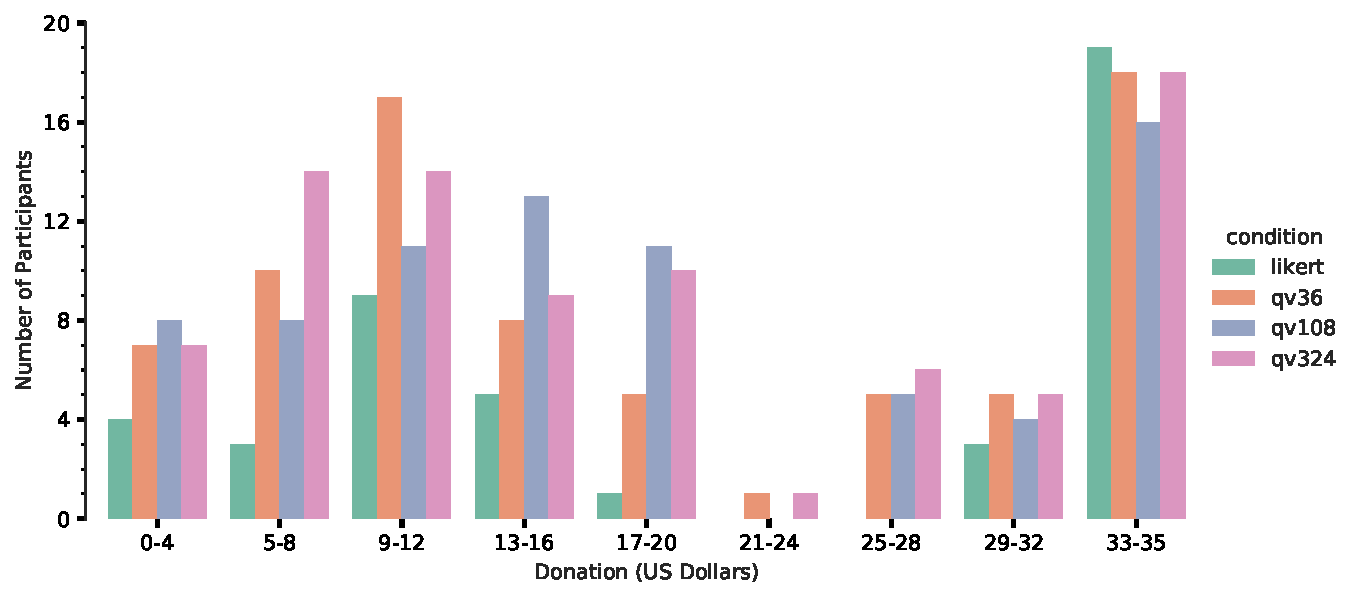
\includegraphics[width=\textwidth, keepaspectratio=true]{content/image/total_contributions_across_conditions.pdf}
    \caption{
       Distributions of the total amount donated by participants across four surveying methods.
       We see two distributions, one centered by $\$9-12$ and the other centered by $\$33$ to $\$35$.
       We also see more Likert participants donate almost most of their donation quota compared to the QV Groups.
    }
    \Description[Distributions of Total Donation Amounts across Groups for experiment 1]{ Distributions of the total amount donated by participants across four surveying methods.
    We see two distributions, one centered by $\$9-12$ and the other centered by $\$33$ to $\$35$.
    We also see more Likert participants donate almost most of their donation quota compared to the QV Groups.}
    \label{fig:total_don_exp1}
\end{figure}

\subsection{QV Budget Usage}
As the number of available voice credits increased, we found no decrease in the median of percentage budget usage -- all around 98\%. QV324 did exhibit a longer tail for percentage budget usage.
\begin{figure}[htpb]
    \centering
    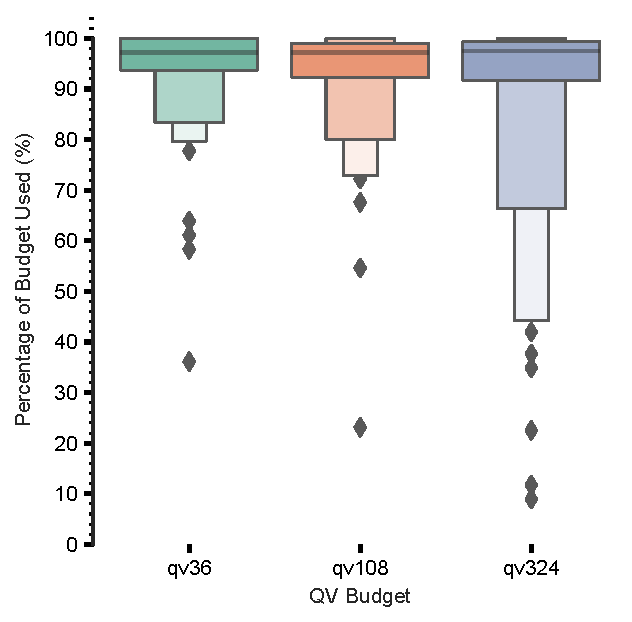
\includegraphics[width=0.5\textwidth, keepaspectratio=true]{content/image/qv_budget_used_distribution.pdf}
    \caption{
      Distribution of Percentage Budget Used in QV36, QV108 and QV324. Percentage budget used is the percentage of voice credits used out of the total voice credits budget available. The medians for all three QVs are around 98\%.
    }
    \Description[Distribution of Percentage Budget Used for experiment 1]{Distribution of Percentage Budget Used for experiment 1}
    \label{fig:qv_budget_exp1}
\end{figure}

\subsection{Posterior Predictive Check}
TO-DO

\section{Experiment 2 Methods}

\subsection{Definition of the Five Video Elements}~\label{elem_def}
In experiment 2, we designed the research scenario to answer the following question: ``Given a video with unsatisfying quality, under limited bandwidth, how should the bandwidth be allocated to enhance the five video and audio elements, including the motion smoothness \cite{huynh2008temporal}, audio stability \cite{hardman1998successful}, audio quality \cite{knoche2008low}, video resolution \cite{knoche2005can}, and audio-video synchronization \cite{steinmetz1996human}, to obtain an acceptable video streaming experience from the viewers' perspective?'' We selected the five video playback elements based on prior work and below are their definitions: 

\begin{itemize}
    \item Motion Smoothness \cite{huynh2008temporal, oeldorf2012bad}: refers to how smooth the visuals of the video are. The number of frames transferred from the server to the viewer per second may be impacted under limited bandwidth. Having a low frame rate means that the video feels jerky and slow.
    \item Audio Stability \cite{hardman1998successful}: refers to how smoothly the audio of the video plays. With limited bandwidth, there may be lost audio packets. This creates short intervals of silence during playback, undermining the interpretability of the audio. The higher probability an audio packet may be lost, the more stuttered the audio sounds.
    \item Video Resolution \cite{oeldorf2012bad, knoche2005can}: refers to how sharp the visuals in the video look. With limited bandwidth, one may reduce the video's size by providing a lower resolution. At a lower resolution, the video imagery becomes pixelated and unclear. 
    \item Audio Quality \cite{oeldorf2012bad, noll1993wideband}: refers to how clear and crisp the audio sounds. A lower audio sampling rate needs lower bandwidth to transmit. With a lower audio sampling rate, the audio sounds more muffled and unclear.
    \item Audio-Video Synchronization \cite{steinmetz1996human}: refers to how well video visuals are matched with the audio playback. Our experiment focused only on the type of asynchronization where the audio plays ahead of the video. Under bandwidth constraint, visuals and audio may be out of sync due to packet loss in visuals or audio.
\end{itemize}

\subsection{Experiment two system design details}
TODO

\section{Experiment Design considerations}
TODO


% not sure if this is needed
\subsection{QV interface iterations}


% draft system design
We designed the QV interface through an iterative design process, with the goal to use visual information to reduce participants' cognitive load. \Cref{fig:qv_donation} shows the body section of the voting panel that contained a list of options to vote on. To the left of each option, participants voted using the plus and minus buttons. Buttons for an item were automatically disabled if the number of voice credits remaining did not permit an additional vote for that item. The number of blue or yellow icons next to the item represented the number of ``for'' and ``against'' votes. We provided participants a bar with percentages to the right of each option, which showed the proportion of voice credits used for that option.  In the summary panel, a progress bar showed the number of voice credits the participants have and have not used out of the total budget. We floated the summary panel at the bottom of the page at anytime to ensure visibility. To prevent environment issues like unstable network connection in client side, we store user’s configuration in browser storage, the user could restore the data when the network resume.

For our experimental system, we used Angular.js and bootstrap for the front-end, Python Flask for the back-end implementation, and MongoDB Atlas for the database. Libraries like Survey.js were adopted to build likert interface. The experimental system source code is publicly available \footnote{https://github.com/a2975667/QV-app}, and so is the code for the standalone QV interface

In this experiment, we build on top of the system for experiment one. Video and audio stabilities were originally adjusted in client browser. The system processes the video frame by frame and pauses some frames according to the probability generated by user’s configuration.  However, low computing power of clients might hinder the stability of video. To prevent unfairness due to devices’ limitation and perform realtime adjustment, videos with different combinations of qualities and levels of motion smoothness were pre-generated ahead by FFMPEG, so were audio files. The precomputed files guarantee the fairness. Even the most distinct environment could fetch the same video and audio. Network environments might results in different video loading time for each client. Thus, we implemented undetermined indicators to distract users’ attention and keep their patientce. The video-audio synchronization was computed by JavaScript. Once the clients detect both files have been loaded, it plays the audio ahead of video according to users’ configuration. This design balances the need for network speed, preventing from streaming every configuration from the server. It also prevents the need for a powerful client such that video and audio qualities were not computed directly on the client. The experiment source code for experiment two is publicly available \footnote{Not yet public}, and so is the video interface as a stand-alone repository.